\chapter{User documentation}
\label{ch:user}

This chapter serves as a user guide to help readers navigate the platform and utilize its features efficiently. By the end of this chapter, users will understand how to create and manage events, interact with the platform as different roles (organizers and attendees), and perform critical actions such as submitting RSVPs, uploading files, and processing payments.

The application is built using Next.js\cite{nextjs} with React\cite{react} for the frontend, leveraging TypeScript\cite{typescript} for type safety and Tailwind CSS\cite{tailwindcss} for responsive and accessible design. The backend utilizes MongoDB\cite{mongodb} as the database, managed through Mongoose\cite{mongoose}, with server-side functionality powered by Next.js API routes. Authentication is handled through Clerk\cite{clerk}, which provides secure session management, role-based access, and OAuth integration. File uploads are managed using Uploadthing\cite{uploadthing}, and payments are integrated with Stripe\cite{stripe} for secure and scalable transaction processing.

Due to the absence of a registered business entity, the application is only available for local deployment, and payment functionalities are demonstrated through mock transactions. While the current setup is sufficient for demonstration purposes, future iterations can include online hosting and live payment processing to make the platform fully operational for real-world use cases.


\section{User Role and Capabilities}
In \textbf{Eventastic}, every user account is designed to support a wide range of capabilities, enabling users to seamlessly act as both event attendees and organizers. This approach simplifies the user experience by allowing a single account to handle all actions related to discovering, participating in, and hosting events.

\subsection{General User Actions}
All users in the system can:
\begin{itemize}
    \item Search for events based on location, date, category, or keywords.
    \item View detailed information about events, including date, time, venue, and ticket options.
    \item Purchase tickets to events or RSVP for free events.
    \item Manage their profile and view a list of registered or upcoming events.
\end{itemize}

\subsection{Event Hosting Capabilities}
In addition to attendee functionalities, users can also create and manage events, effectively acting as organizers. These capabilities include:
\begin{itemize}
    \item Creating and publishing events by filling out forms with event titles, descriptions, locations, dates, ticket pricing, and images.
    \item Managing ticket sales, tracking RSVPs, and viewing attendee details in real-time.
    \item Editing event details or canceling events when necessary.
    \item Sending notifications or updates to registered attendees.
    \item Accessing analytics and insights to evaluate event performance, such as ticket sales, attendance trends, and other metrics.
\end{itemize}

\subsection{Unified User Experience}
Since every account supports both attendee and organizer functionalities, there is no need for separate accounts. Users can seamlessly switch between discovering events to attend and managing events they organize. This unified design ensures that users have all the tools they need to participate in or host events without additional complexity.

\textit{Note:} The terms \textbf{User}, \textbf{Attendee}, and \textbf{Organizer} are used interchangeably throughout this documentation, as they all refer to a single account type with extended capabilities based on user actions.






\section{Software Requirements and How to Start the
Program}

To host the website locally, the user must have \textbf{Node.js}\cite{nodejs} installed
in advance. This software is a popular runtime JavaScript environment, used to run
the JavaScript\cite{javascript} projects of any kind. Along with Node.js, the installation will also set
up \textbf{Node Package Manager (npm)}\cite{npm}. By using this package
manager, the user can add, remove or update packages necessary for the project.
The official installation guide can be found at \textit{https://nodejs.org/en/learn/getting-started/how-to-install-nodejs}

After installation, one can verify by following these steps.

\begin{itemize}
	\item Open a terminal or a command prompt depending on your operating system.
	\item Type \textit{node -v} and \textit{npm -v} and press Enter. This Figure~\ref{fig:terminal-1} shows a successful
installation of Node.js program. The versions of the software can be seen as a
result.
\end{itemize}



\begin{figure}[H]
	\centering
	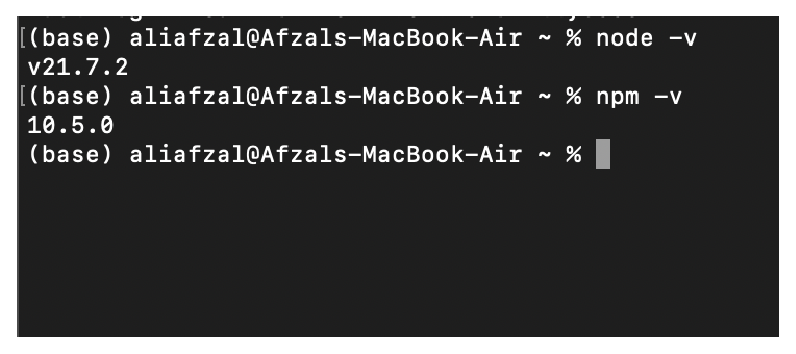
\includegraphics[width=0.6\textwidth,height=100px,frame]{images/terminal1.eps}
	\caption{How to Verify Node.js Installation}
        \label{fig:terminal-1}
\end{figure}


Run the following command from the root directory in order to  install the dependencies :

\lstset{caption={Install Packages Command}}
\begin{lstlisting}
npm install
\end{lstlisting}


The next step involves setting up environment variables, create a new file named \textit{.env} in the root of your project and add the following content:
\lstset{caption={.env file contents}}
\begin{lstlisting}
#NEXT
NEXT_PUBLIC_SERVER_URL=

#CLERK
NEXT_PUBLIC_CLERK_PUBLISHABLE_KEY=
CLERK_SECRET_KEY=
NEXT_CLERK_WEBHOOK_SECRET=

NEXT_PUBLIC_CLERK_SIGN_IN_URL=/sign-in
NEXT_PUBLIC_CLERK_SIGN_UP_URL=/sign-up
NEXT_PUBLIC_CLERK_AFTER_SIGN_IN_URL=/
NEXT_PUBLIC_CLERK_AFTER_SIGN_UP_URL=/

#MONGODB
MONGODB_URI=

#UPLOADTHING
UPLOADTHING_SECRET=
UPLOADTHING_APP_ID=

#STRIPE
STRIPE_SECRET_KEY=
STRIPE_WEBHOOK_SECRET=
NEXT_PUBLIC_STRIPE_PUBLISHABLE_KEY=
\end{lstlisting}

Replace the placeholder values with your actual credentials.

Next, run the following command and open \textit{http://localhost:3000} in your browser to view the project.
\lstset{caption={Install Packages Command}}
\begin{lstlisting}
npm run dev
\end{lstlisting}


\section{Features}

This part of the documentation entails the features of our website. The readers
will understand the usage of each web component after this section.


\subsection{Common Features}

The common features are the ones which appear in most of the pages. They
include components like header, navigation bar, profile menu and footer. See Figure~\ref{fig:header}

\begin{figure}[H]
	\centering
	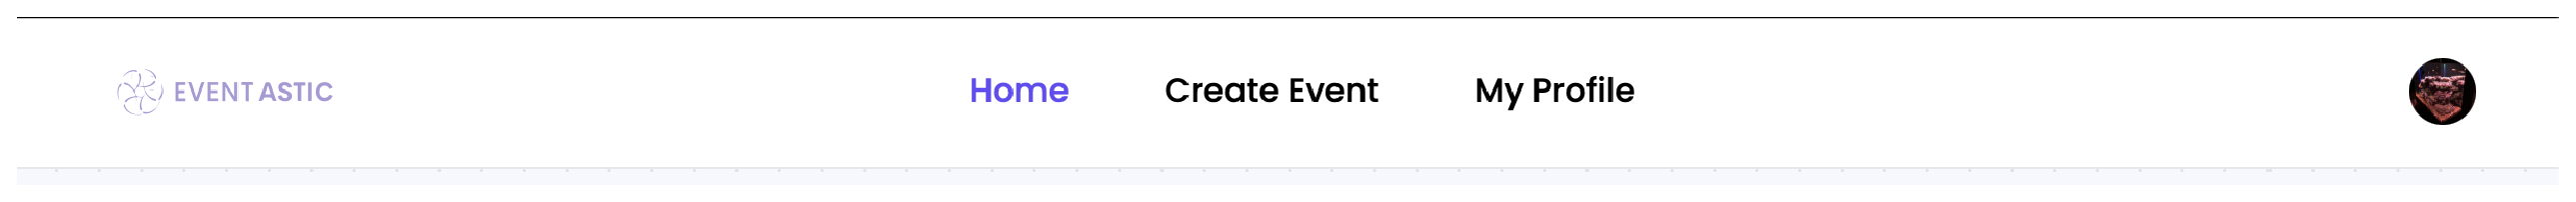
\includegraphics[width=1.0\textwidth,height=40px,frame]{images/header.eps}
	\caption{Header and Navigation Bar}
        \label{fig:header}
\end{figure}



Profile menu can be activated by clicking on the user icon in the navigation
bar. Figure~\ref{fig:profile} shows a list of account related menu for the user.

\begin{figure}[H]
	\centering
	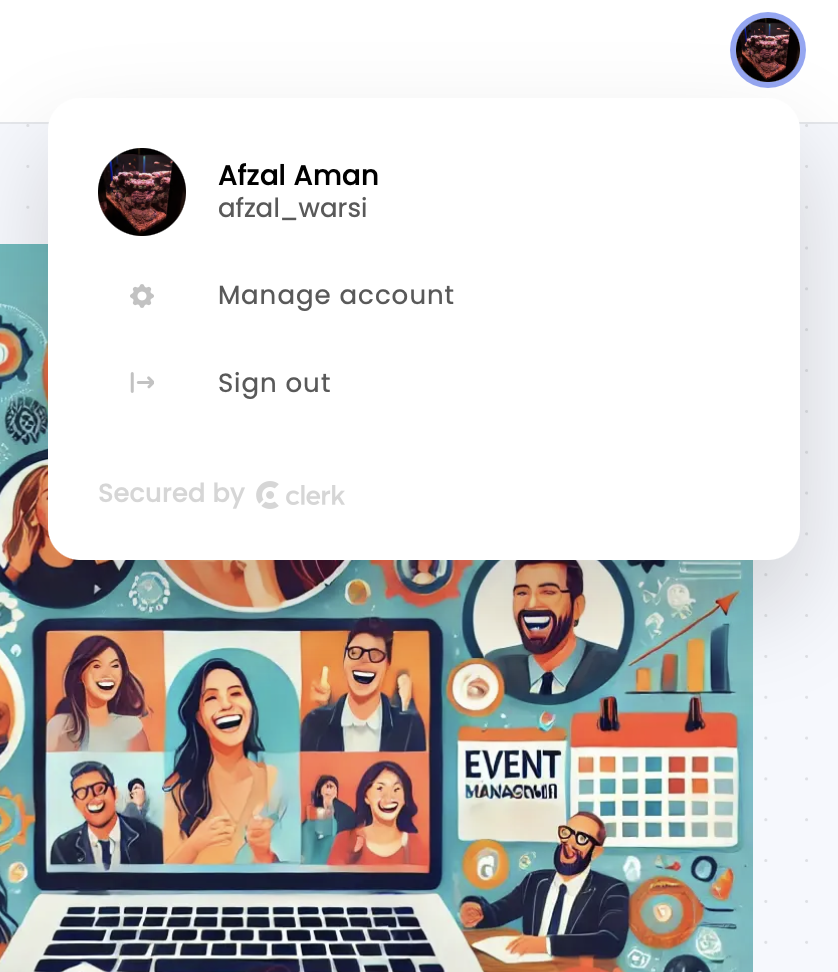
\includegraphics[width=0.6\textwidth,height=250px,frame]{images/profile.png}
	\caption{Profile Menu}
        \label{fig:profile}
\end{figure}

From this menu, the users can register, log in or log out from their accounts, or
manage their profiles.

\begin{figure}[H]
	\centering
	
\includegraphics[width=1.0\textwidth,height=40px,frame]{images/footer.png}
	\caption{footer}
        \label{fig:footer}
\end{figure}

\subsection{Registration}

The Register link in the profile menu will redirect the user to the Register page.
The user must fill out the form and complete the process by clicking the register
button. The user can also choose to register via \textbf{Google}. The information needed is as shown in Figure~\ref{fig:register}

\begin{figure}[H]
	\centering	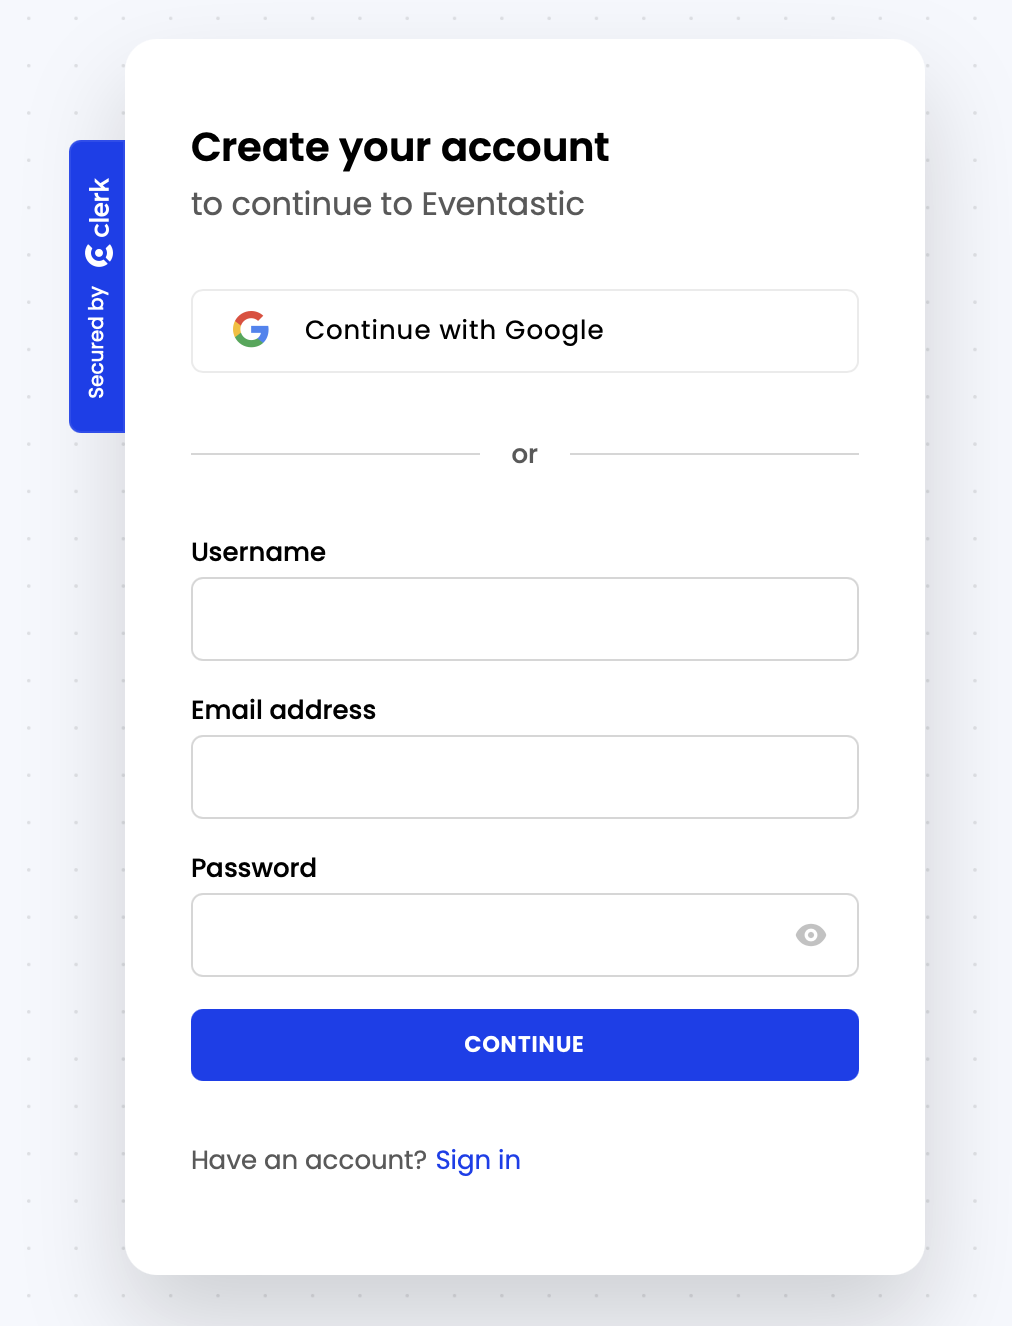
\includegraphics[width=0.6\textwidth,height=300px,frame]{images/register.png}
	\caption{User Registration Form}
        \label{fig:register}
\end{figure}


\subsection{Logging In}


After a successful registration, users will be taken to the login page. They can
either log in there or manually by activating the profile menu and using the link
there instead, see Figure~\ref{fig:login}. Once clicked on \textit{continue}, the user will be prompted to enter the password.

\begin{figure}[H]
	\centering	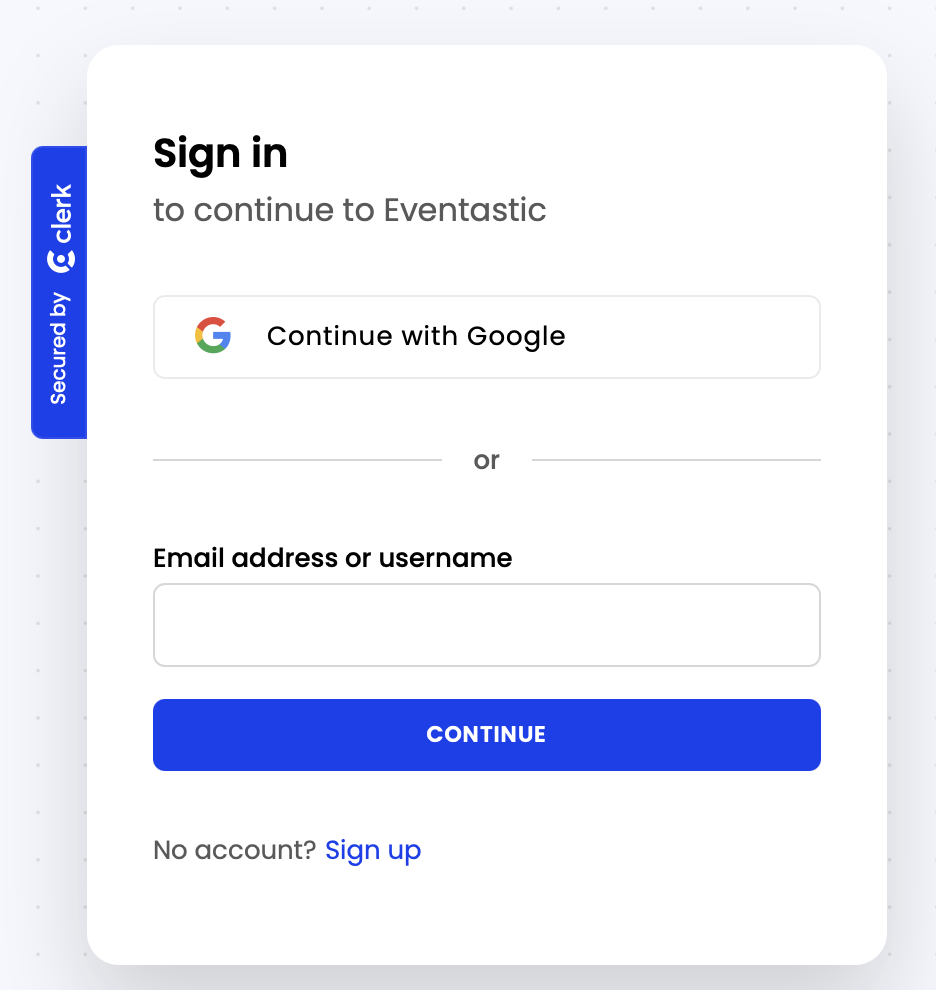
\includegraphics[width=0.6\textwidth,height=300px,frame]{images/login.png}
	\caption{User Registration Form}
        \label{fig:login}
\end{figure}


\subsection{My Profile}
The \textbf{My Profile} page in \textbf{Eventastic} serves as a central hub for users to manage both their purchased tickets and the events they organize. This section provides an overview of the key functionalities available on the profile page see Figure~\ref{fig:profile1} below.

\begin{figure}[H]
	\centering	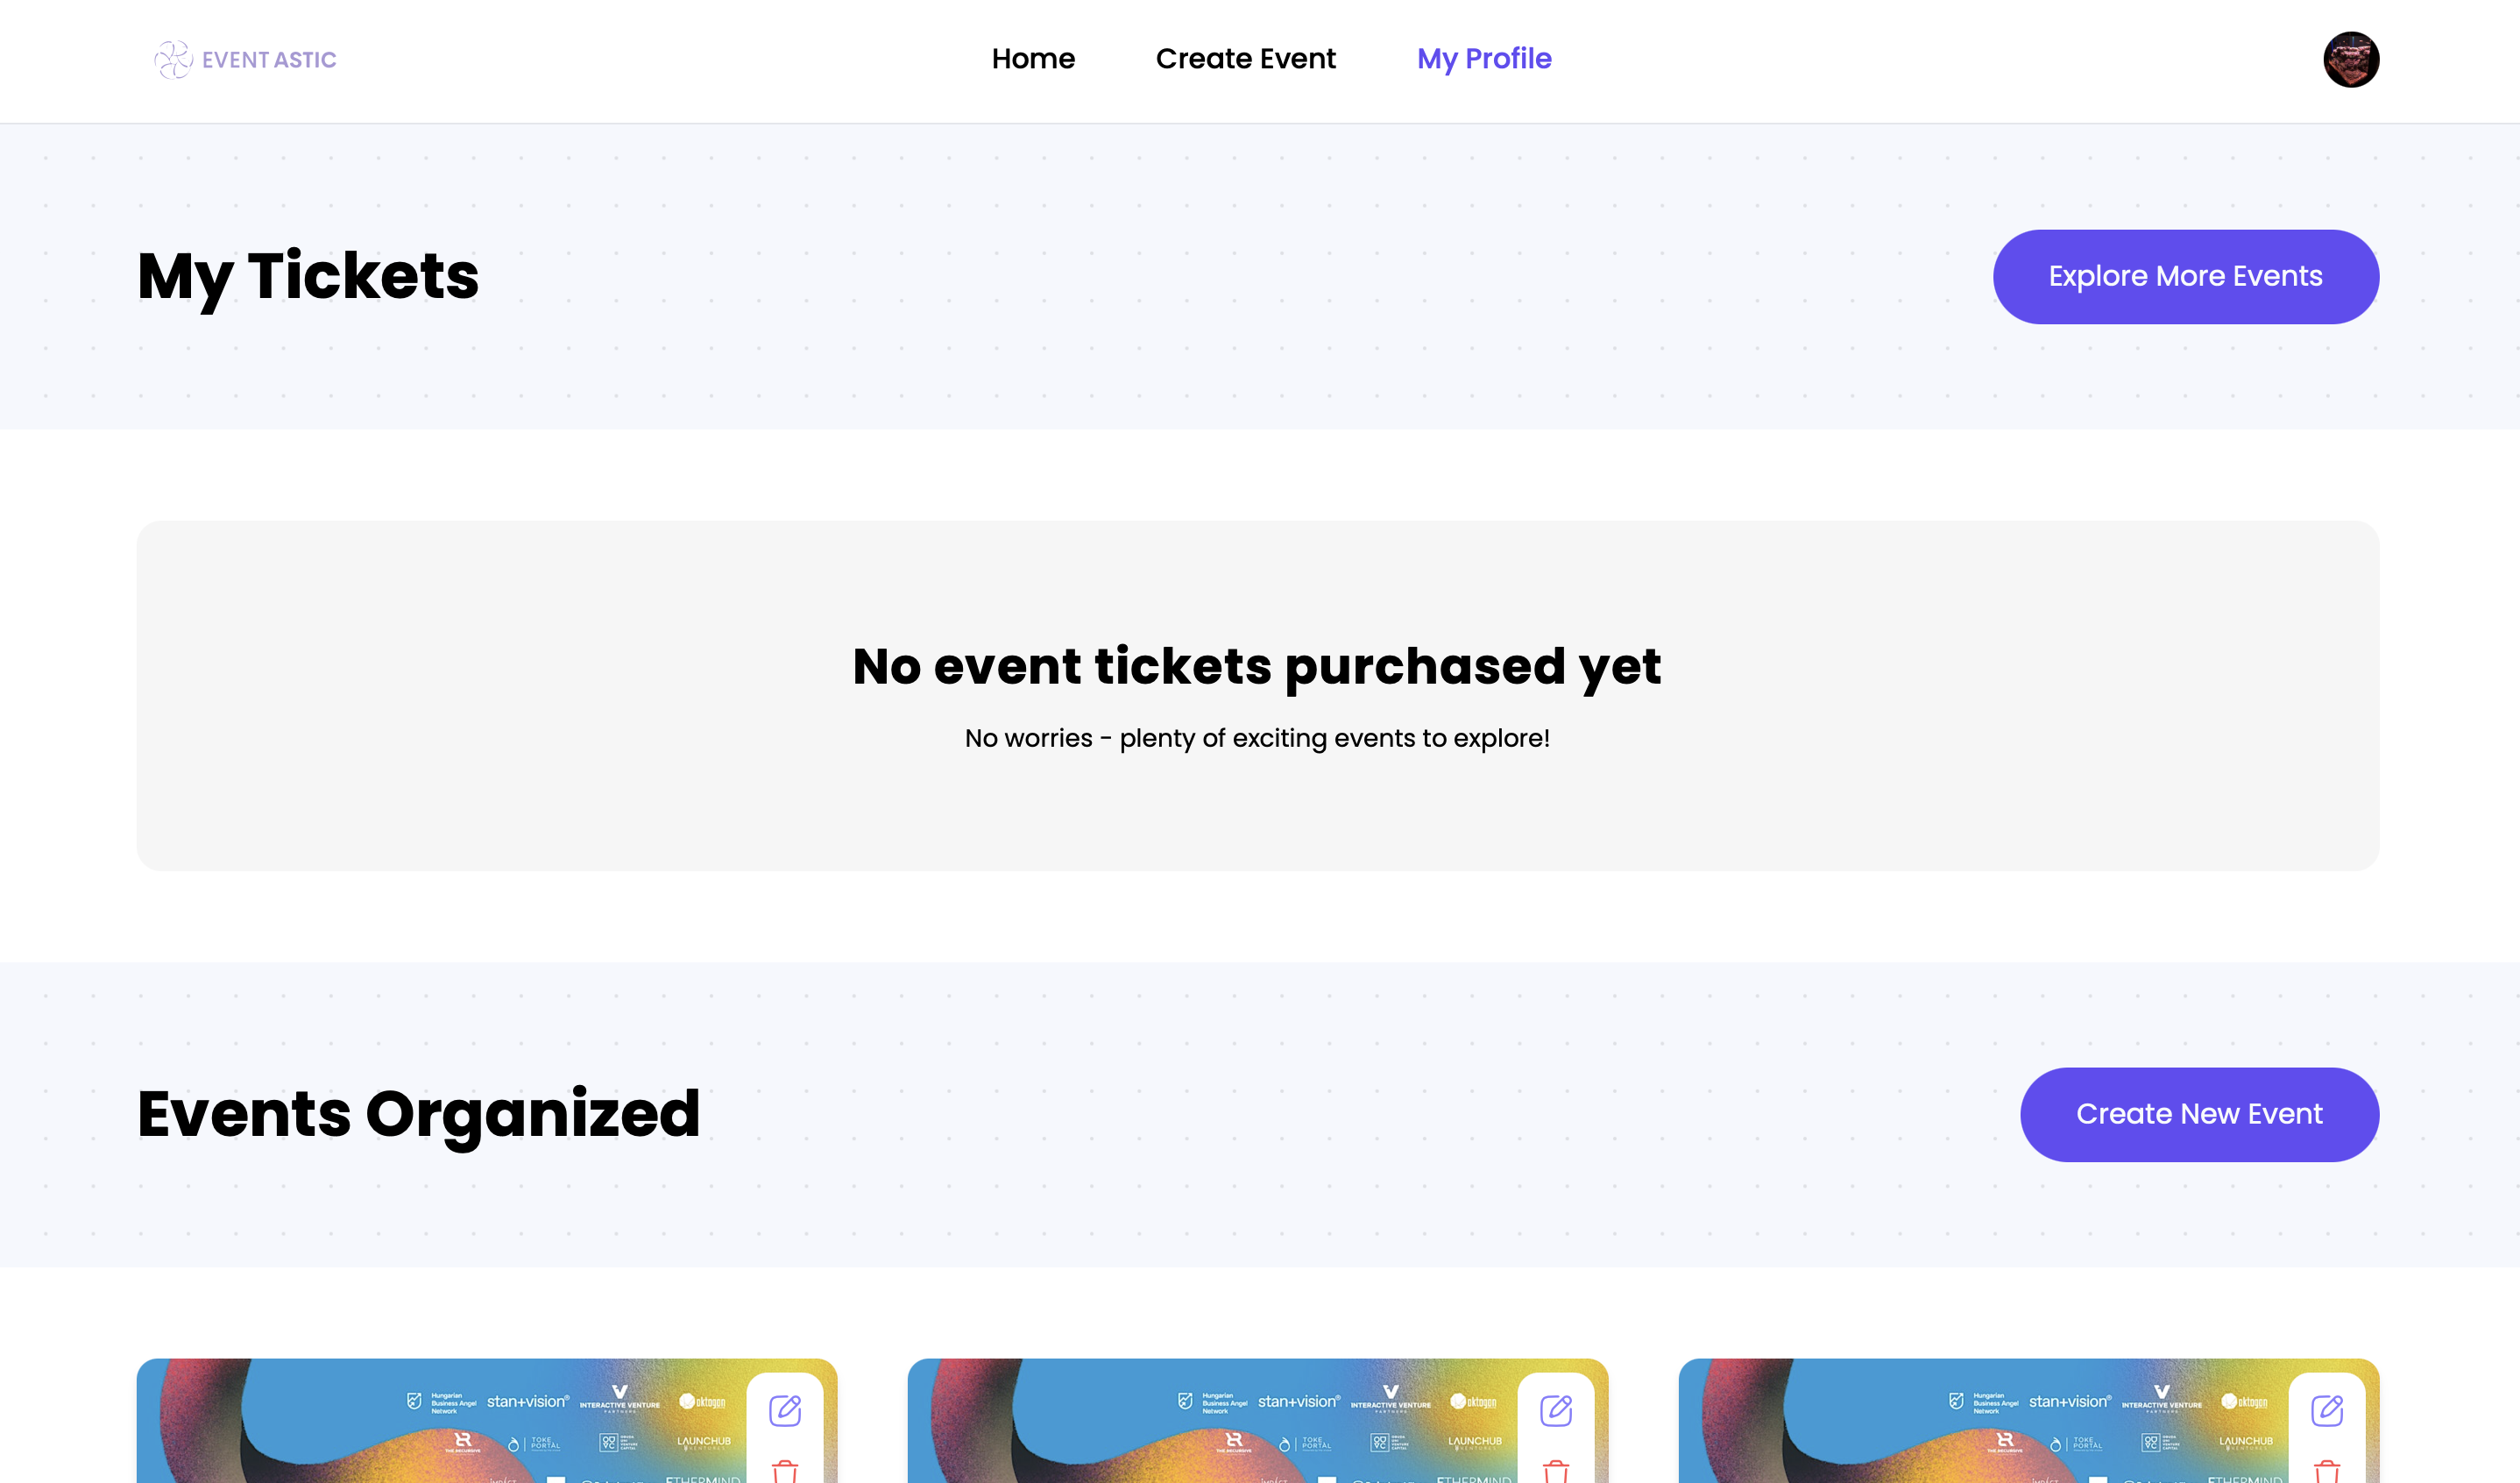
\includegraphics[width=1.0\textwidth,height=300px,frame]{images/profile1.png}
	\caption{My Profile Page 1}
        \label{fig:profile1}
\end{figure}

The \textbf{My Tickets} section displays a comprehensive list of all events for which the user has either purchased tickets or submitted an RSVP. Each event in this list is clickable, allowing users to navigate directly to the corresponding event page. On the event page, users can view detailed information about the event, including the date, time, location, and other relevant details.

\begin{figure}[H]
	\centering	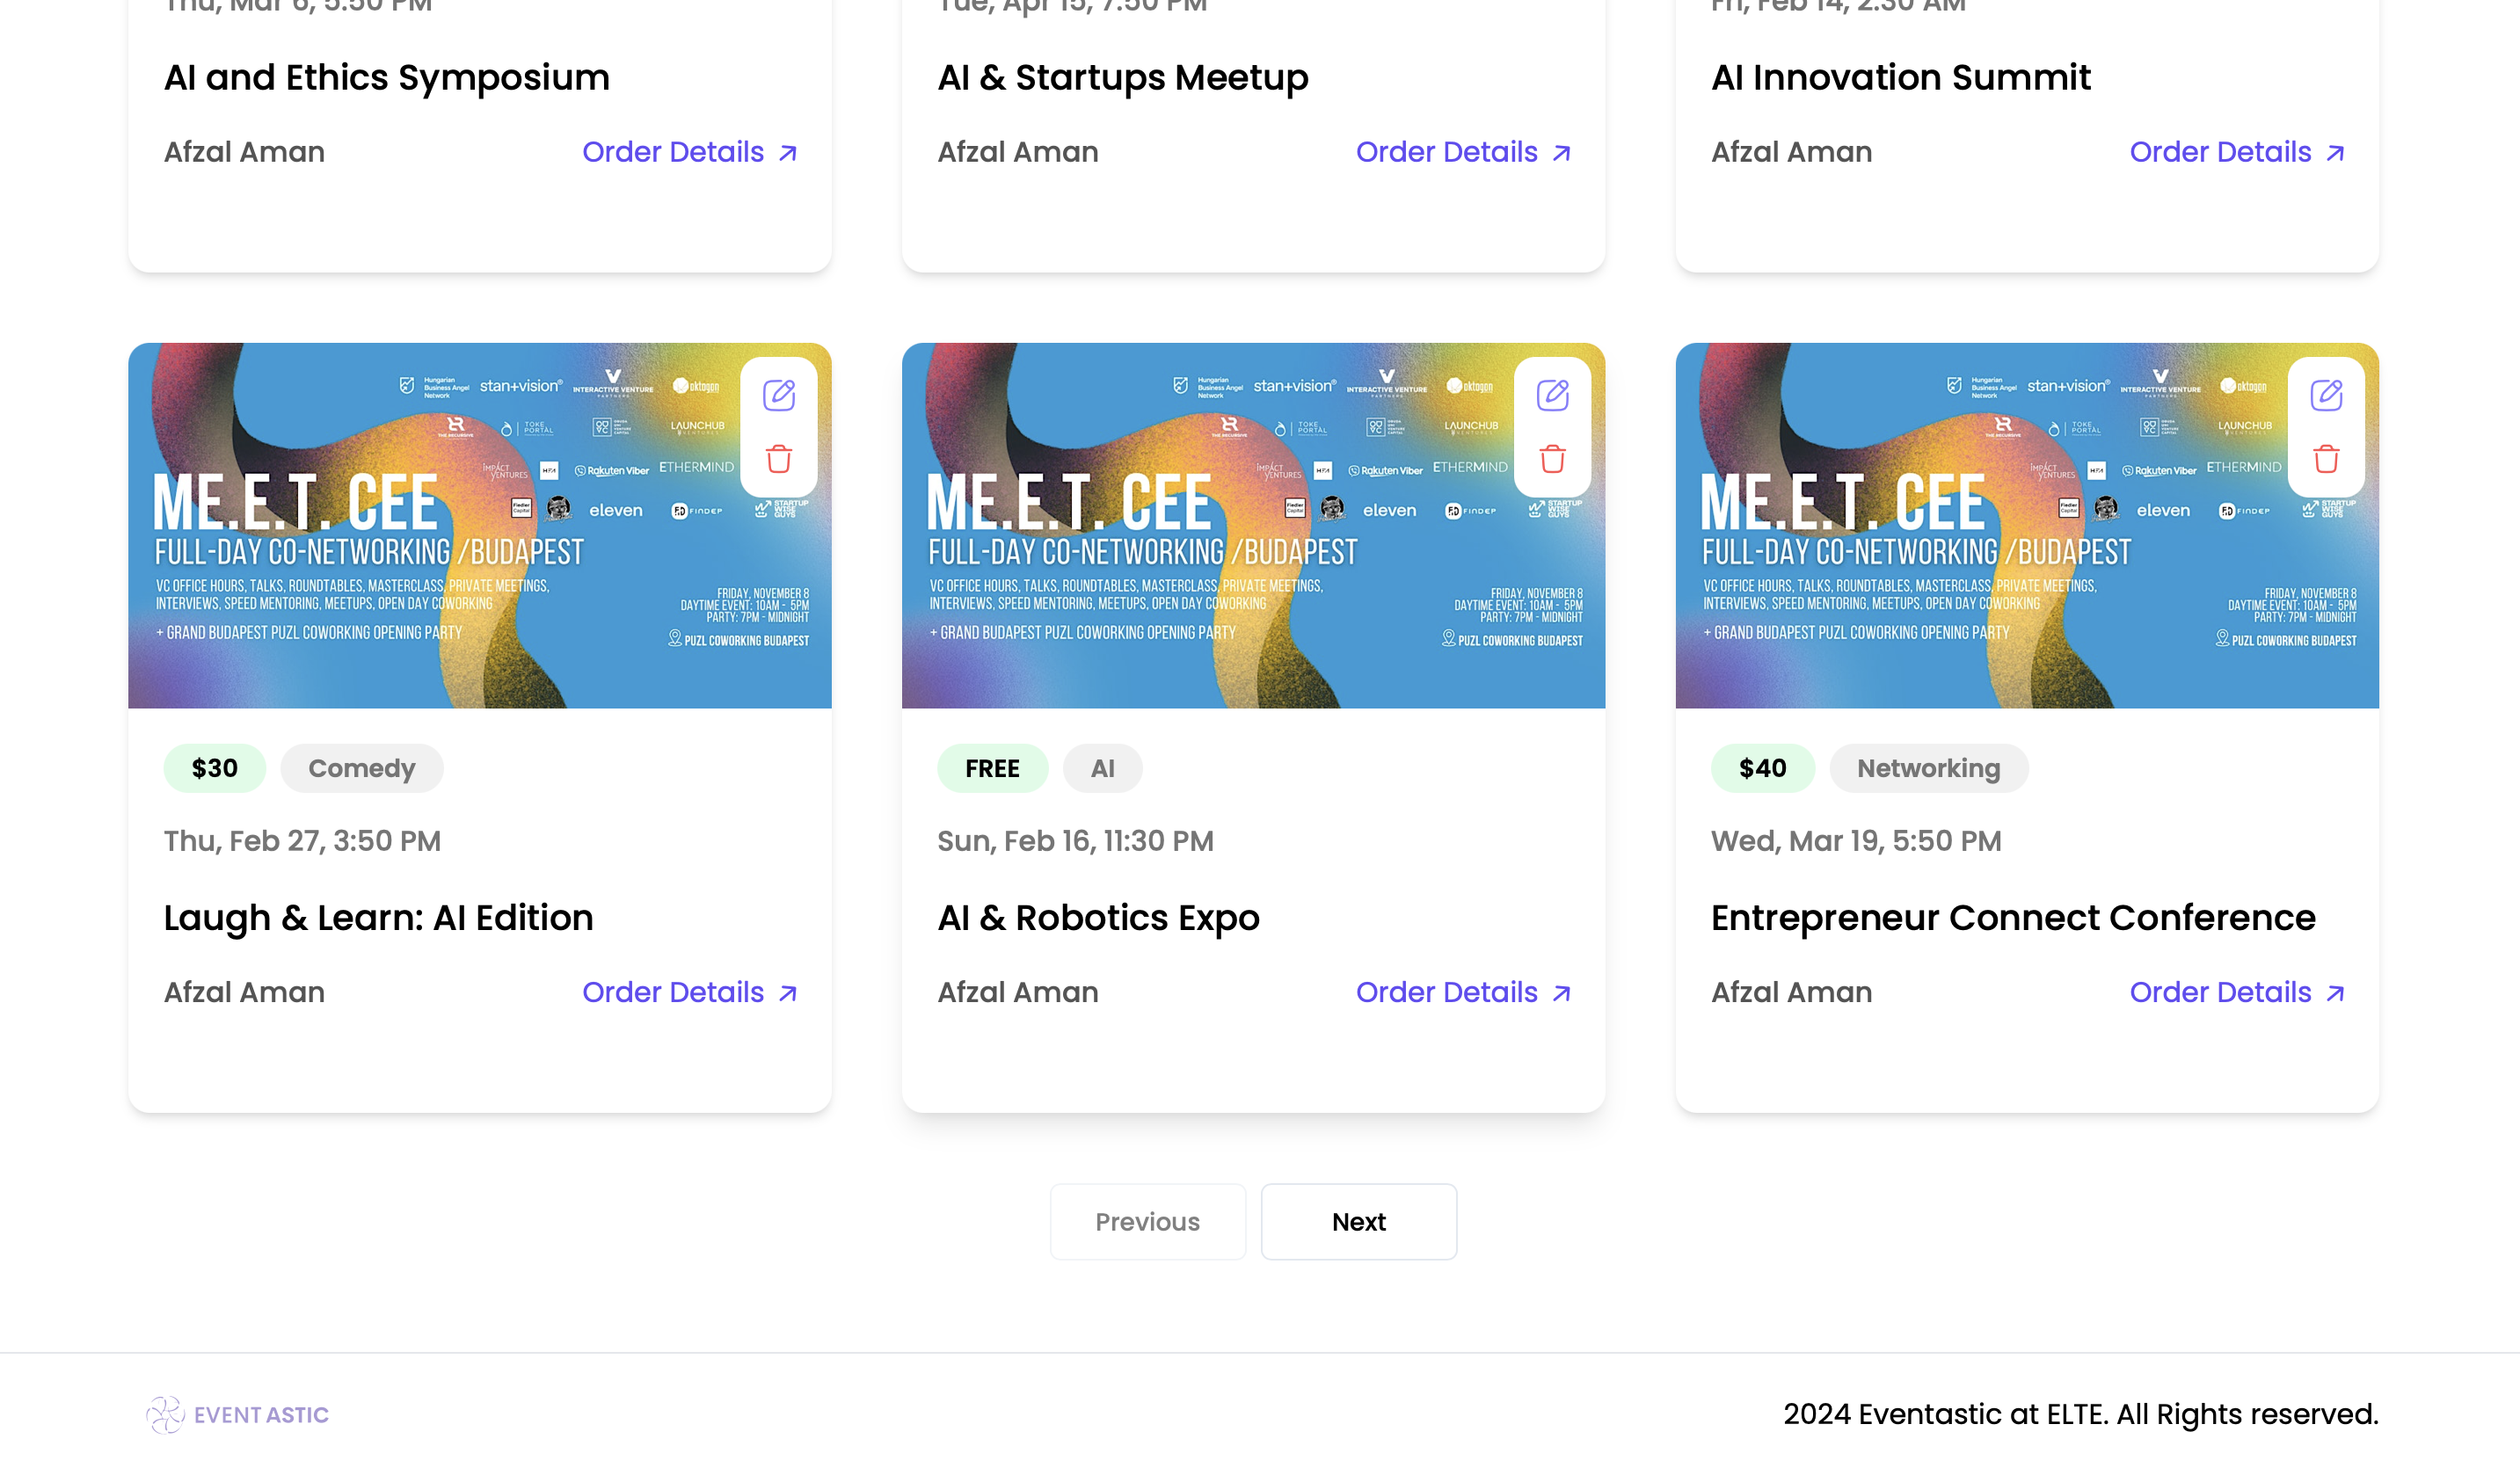
\includegraphics[width=1.0\textwidth,height=300px,frame]{images/profile2.png}
	\caption{My Profile Page 2}
        \label{fig:profile2}
\end{figure}


The \textbf{Events Organized} section (see Figure~\ref{fig:profile2}) provides users with a list of all the events they have created. For each event in this list, the following options are available:
\begin{itemize}
    \item \textbf{Edit Event:} Allows users to modify the event details such as title, description, date, time, location, ticket pricing, or other event-specific information.
    \item \textbf{Delete Event:} Enables users to permanently remove an event from the platform if it is no longer needed.
    \item \textbf{Order Details:} This button provides users with an overview of all the attendees and order details associated with the event. This feature is particularly useful for organizers to track ticket sales, RSVPs, and attendee information efficiently.
\end{itemize}

\textbf{My Profile} ensures that users can manage their interactions with the platform, whether they are attending events or organizing them, all from a single, intuitive interface.



\subsection{Event Search and Filtering}

\begin{figure}[H]
	\centering	
\includegraphics[width=1.0\textwidth,height=80px,frame]{images/search1.png}
	\caption{Search filter}
        \label{fig:search1}
\end{figure}

\textbf{Eventastic} provides an intuitive and efficient event search functionality to help users quickly find events of interest. 

Users can search for events by simply entering the event name in the search bar see Figure~\ref{fig:search1} above. The search process is dynamic and happens in real time, displaying matching results as the user types. This ensures a seamless and responsive experience, allowing users to locate specific events effortlessly.

To enhance the search functionality, a filtering system is implemented. Users can refine their search results by specifying the \textbf{category} of the event. This feature enables a more targeted search, ensuring that users can easily discover events that match their preferences and interests.


\begin{figure}[H]
	\centering	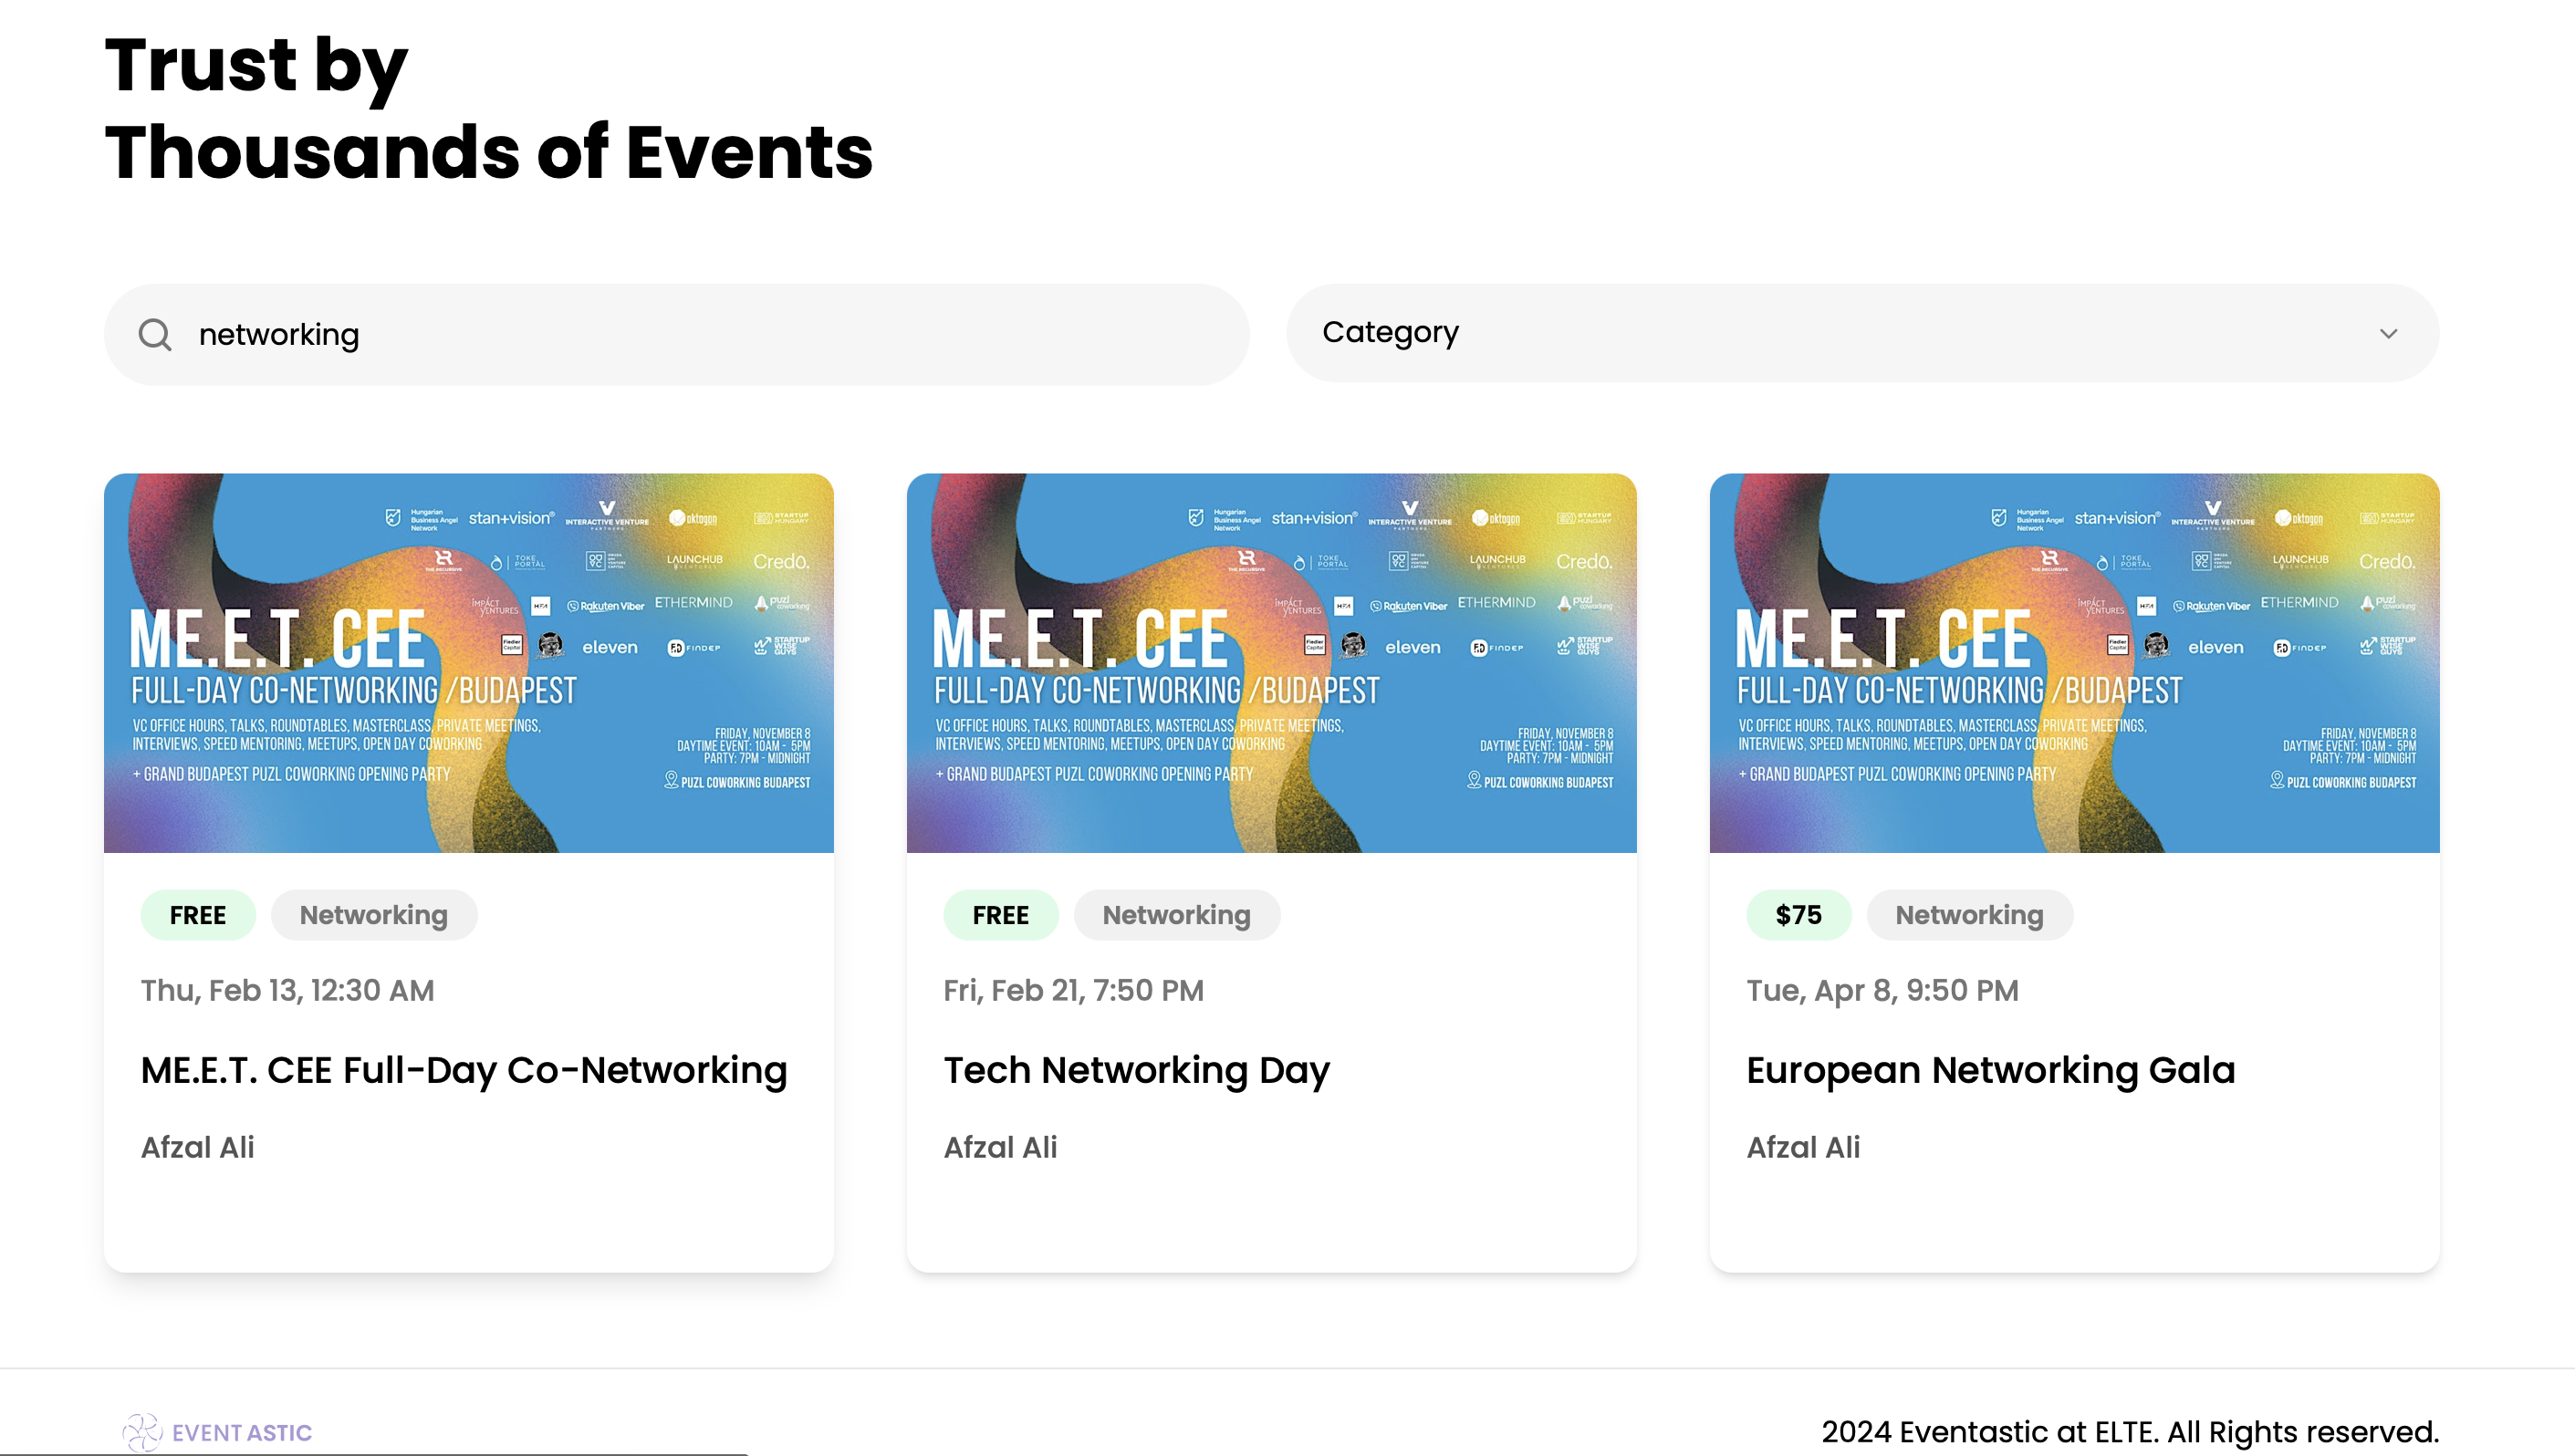
\includegraphics[width=1.0\textwidth,height=300px,frame]{images/search2.png}
	\caption{Search Event Result}
        \label{fig:search2}
\end{figure}


The combination of real-time search and category filtering ensures a user-friendly and efficient event discovery process, catering to the diverse needs of the platform’s users.


\subsection{Event Page}

The \textbf{Event Page} in \textbf{Eventastic} provides users with comprehensive details about each event. It is designed to deliver all essential information at a glance, ensuring users can make informed decisions about their participation. 

The event page displays all relevant details about the event, including:
\begin{itemize}
    \item \textbf{Cost:} Ticket pricing or indication if the event is free.
    \item \textbf{Category:} The type of event (e.g., music, workshop, seminar).
    \item \textbf{Organizer Details:} Information about the event organizer.
    \item \textbf{Location:} Venue or online meeting link for the event.
    \item \textbf{Start and End Date/Time:} Precise timing of the event.
    \item \textbf{Description:} A detailed description providing an overview of the event.
    \item \textbf{External Links:} Additional resources or references for the event.
\end{itemize}

\begin{figure}[H]
	\centering	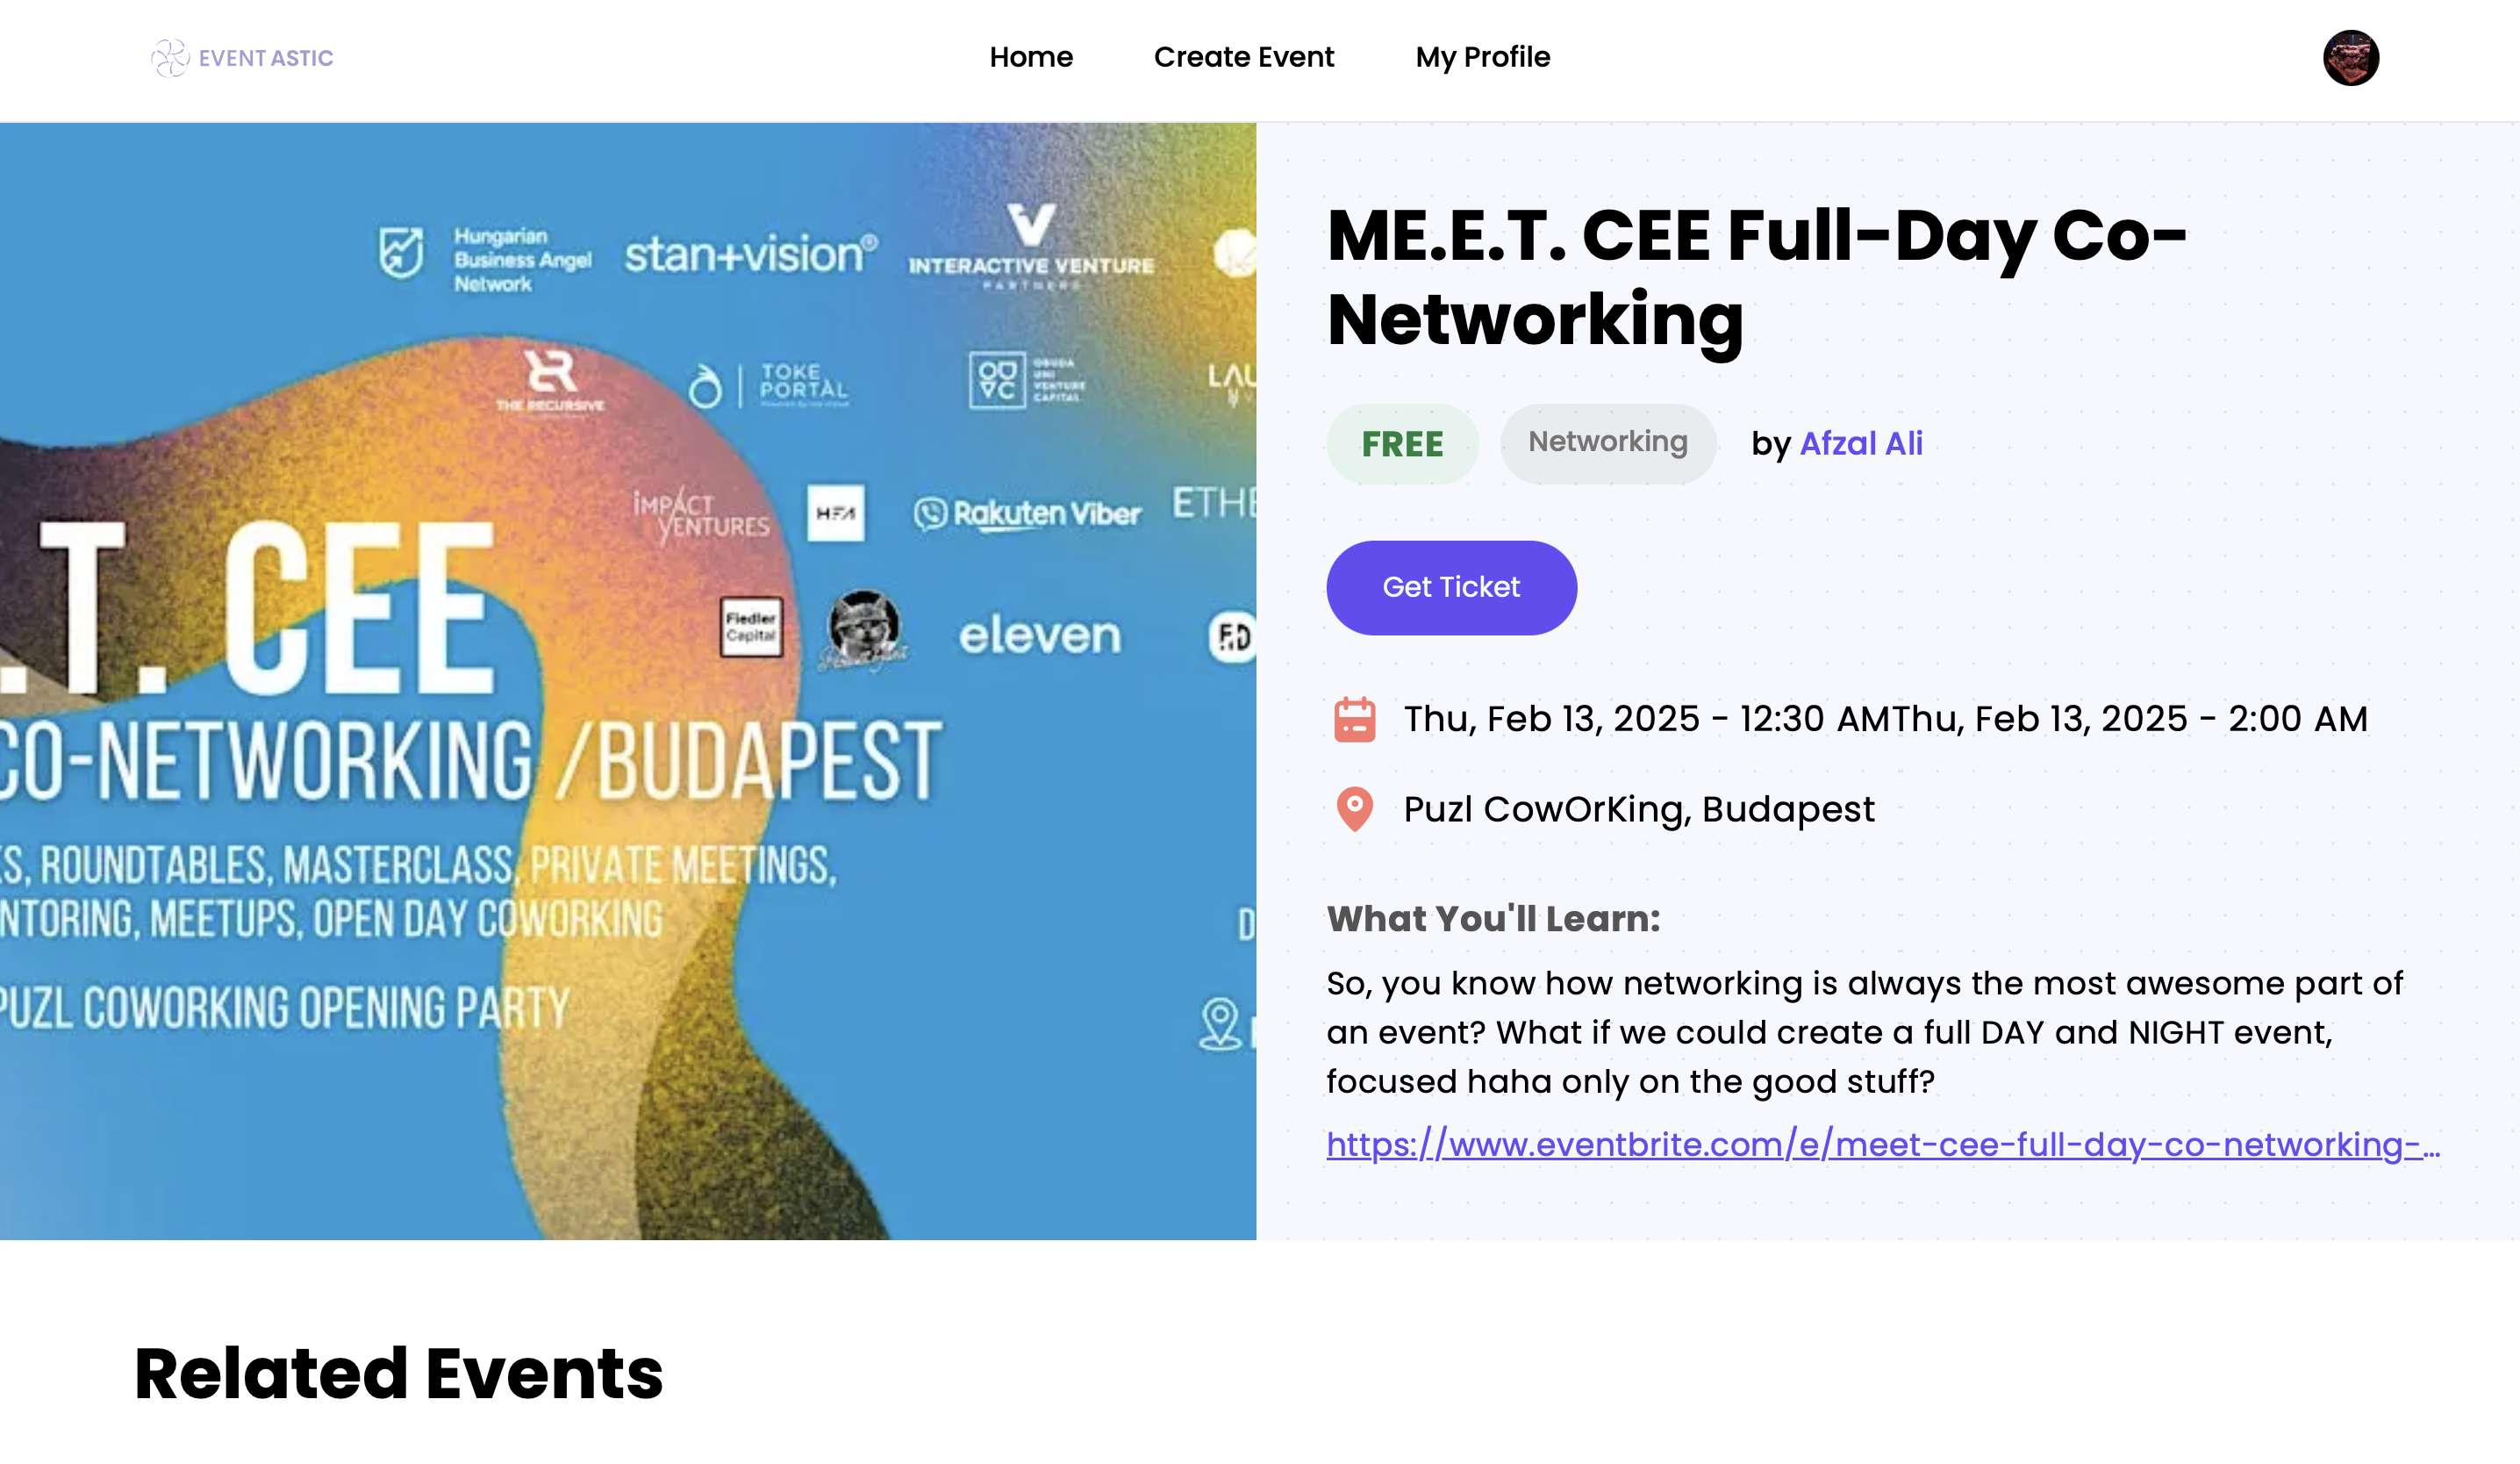
\includegraphics[width=1.0\textwidth,height=300px,frame]{images/event.png}
	\caption{Event Page}
        \label{fig:event}
\end{figure}

The page includes a prominent \textbf{"Get Ticket"} button, allowing users to seamlessly purchase tickets or RSVP for the event directly from the page.

At the bottom of the event page, users can discover \textbf{Related Events}, which are recommendations based on similar categories or user preferences. This feature enhances event discovery and encourages further engagement on the platform.

The event page is designed to provide a rich and user-friendly experience, presenting all critical information in a structured and visually appealing manner.


\subsection{Checkout Process}
The \textbf{Checkout Process} in \textbf{Eventastic} is streamlined to provide users with a seamless experience when purchasing event tickets. 

When a user wishes to purchase a ticket for an event, they can click the \textbf{Buy Ticket} button available on the event page. This action redirects the user to the \textbf{Stripe Payment Gateway} see Figure~\ref{fig:checkout} below , where the transaction is processed.


\begin{figure}[H]
	\centering	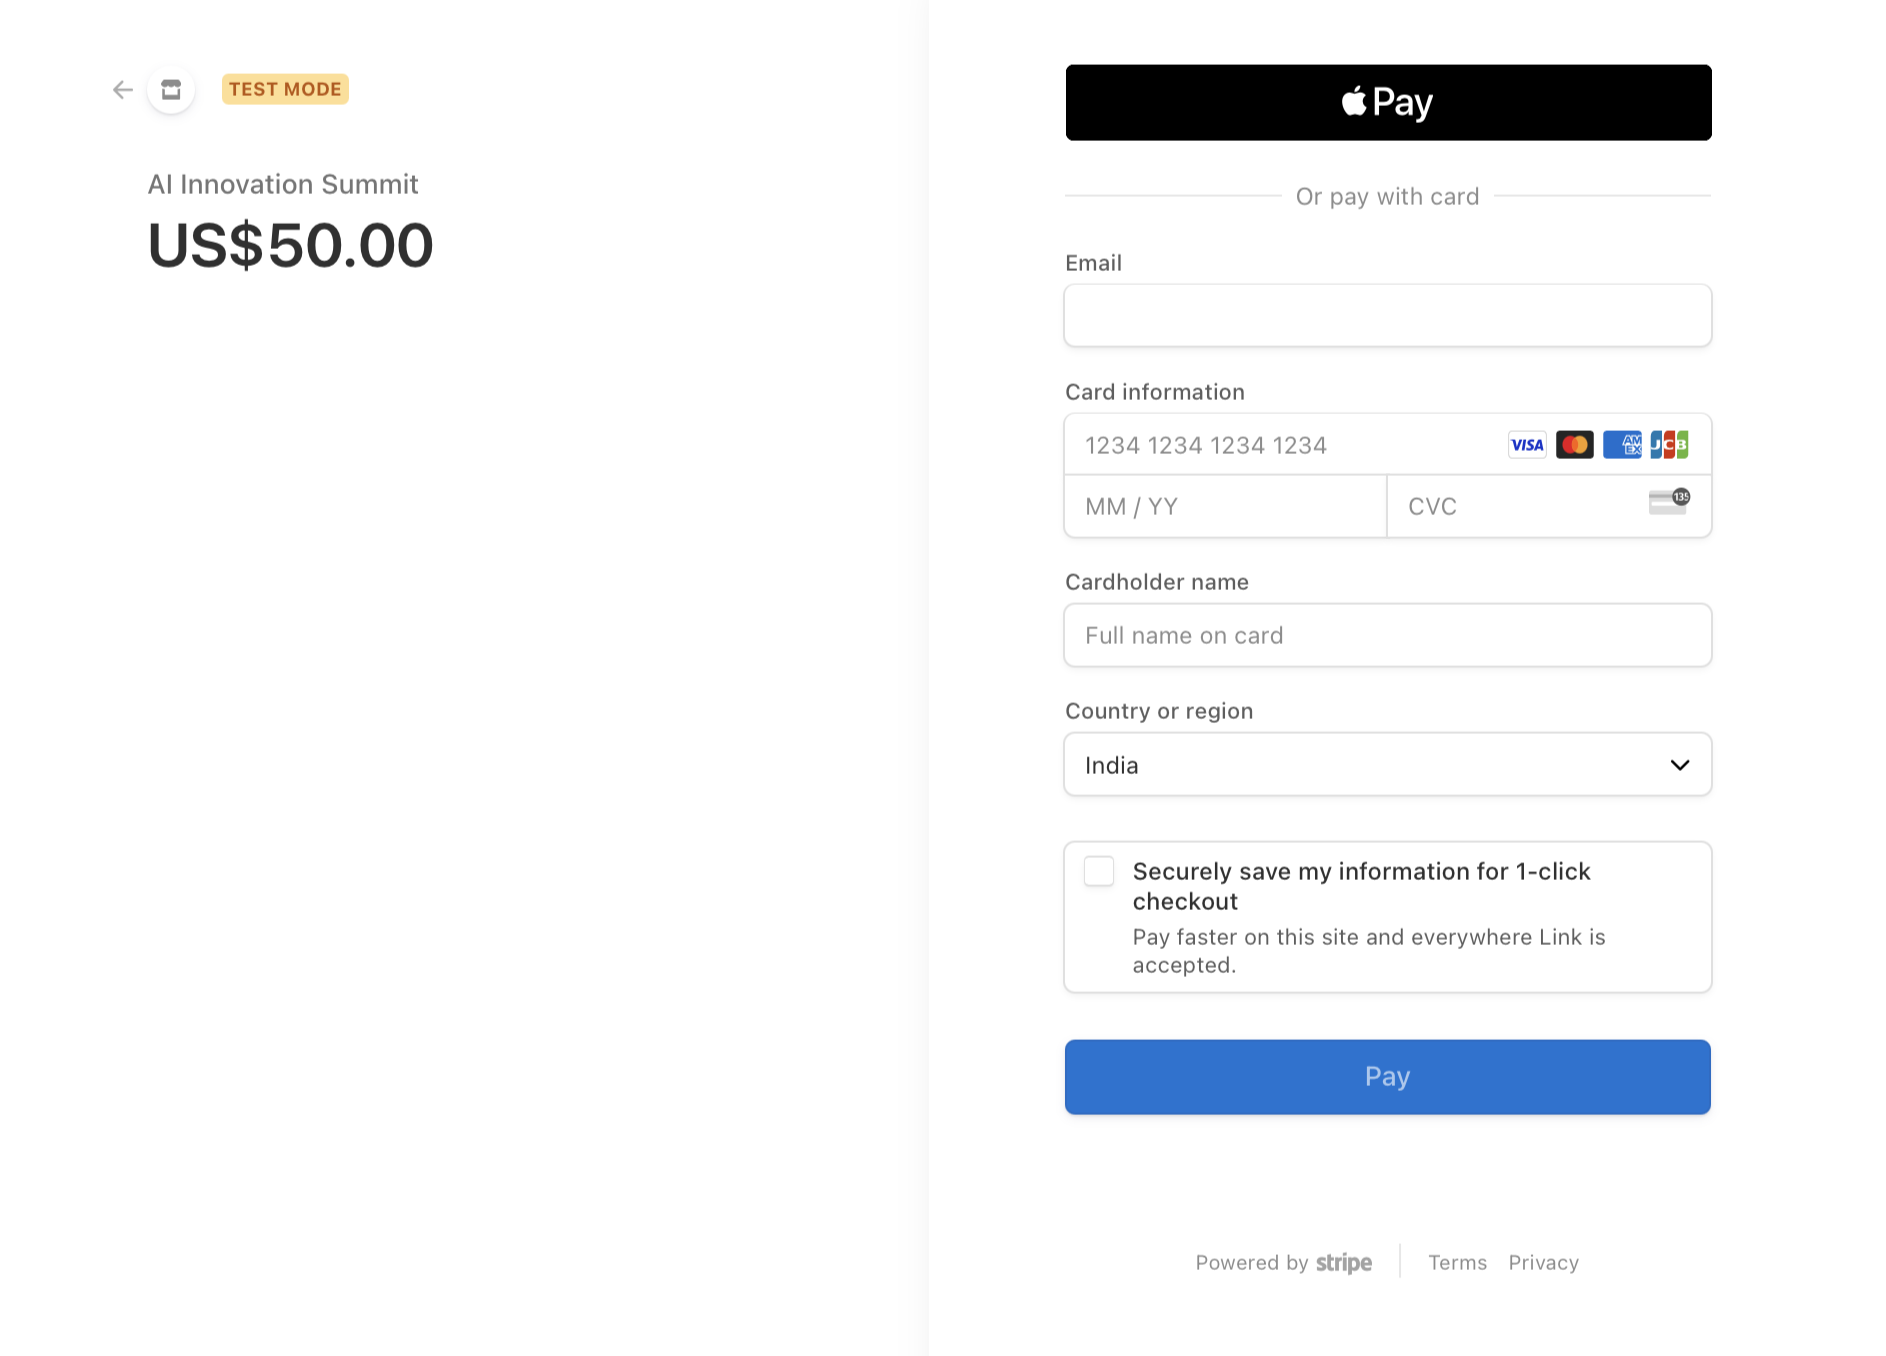
\includegraphics[width=1.0\textwidth,height=300px,frame]{images/checkout.png}
	\caption{Checkout Page}
        \label{fig:checkout}
\end{figure}

Since the platform operates in \textbf{test mode}, users are required to follow the \textbf{test payment routine} to simulate transactions. Stripe provides a variety of test card credentials for this purpose. Users can refer to the official \href{https://stripe.com/docs/testing}{Stripe Documentation} for a comprehensive list of test card options. 

For example, using the card number \texttt{4242 4242 4242 4242} with any valid expiration date and CVV will simulate a successful transaction.

There is also an option for \textbf{Apple Pay} or \textbf{Google Pay} depending on the user's operating system.

Upon completing the payment, the user is automatically redirected back to the platform. The result of the transaction is displayed on the confirmation page:
\begin{itemize}
    \item For \textbf{successful payments}, a confirmation message is shown, indicating that the ticket purchase was successful.
    \item For \textbf{failed payments}, an error message is displayed, informing the user of the issue.
\end{itemize}

This process ensures a user-friendly and secure payment experience while enabling developers and testers to simulate real-world scenarios effectively.


\subsection{Creating an Event}
The \textbf{Create Event} feature allows users to host and publish their events on the \textbf{Eventastic} platform seamlessly.

To create an event, the user can simply click on the \textbf{Create Event} button located in the navigation bar. This action opens a comprehensive event creation form.


The event creation form requires the user to input essential details about the event, including:
\begin{itemize}
    \item \textbf{Event Title:} A descriptive title for the event.
    \item \textbf{Description:} Detailed information about the event.
    \item \textbf{Location:} The venue or link for the event.
    \item \textbf{Start and End Dates/Times:} The schedule for the event.
    \item \textbf{Ticket Price:} Cost of tickets (or mark the event as free).
    \item \textbf{External Links:} Optional links, such as additional resources or social media.
    \item \textbf{Category:} Choose an appropriate category from the existing list or add a new one if needed.
\end{itemize}

If the user wishes to create a new event category beyond the available options, the form provides an easy-to-use \textbf{Add Category} feature see Figure~\ref{fig:createEvent2} below. This ensures flexibility in categorizing events appropriately.

Once all the required details are filled out, the user can click the \textbf{Create Event} button at the bottom of the form. This action instantly makes the event live on the platform, allowing it to be viewed and accessed by other users.

The event creation page is designed for simplicity and efficiency, ensuring users can create events quickly while providing all necessary details. A visual example of the form is shown in Figure~\ref{fig:createEvent1}.

\begin{figure}[H]
	\centering	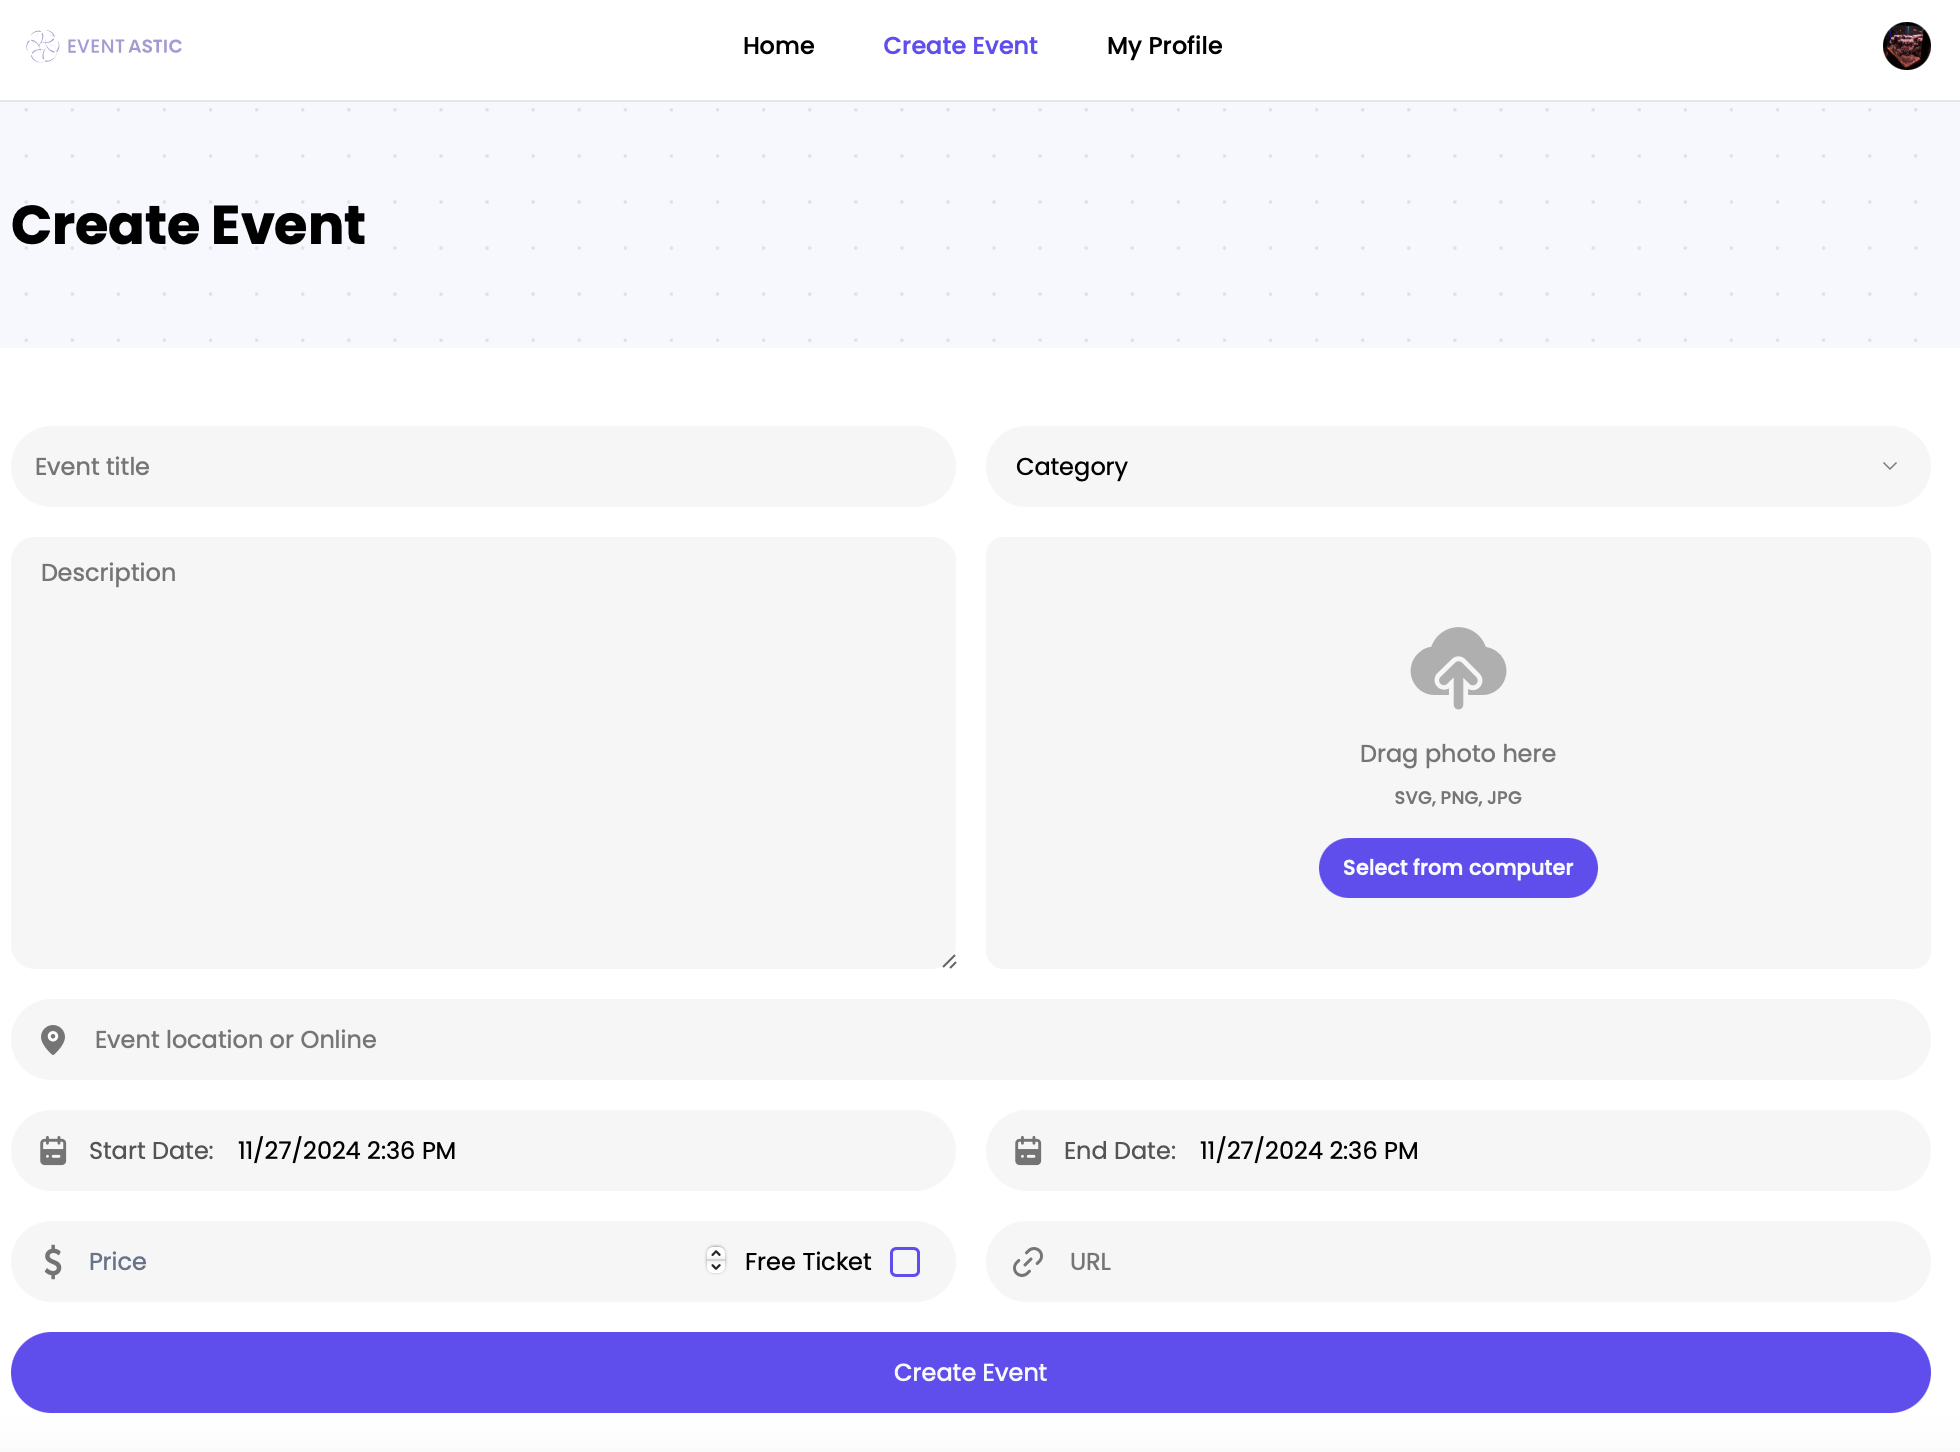
\includegraphics[width=1.0\textwidth,height=300px,frame]{images/createEvent1.png}
	\caption{Create Event Page}
        \label{fig:createEvent1}
\end{figure}


\begin{figure}[H]
	\centering	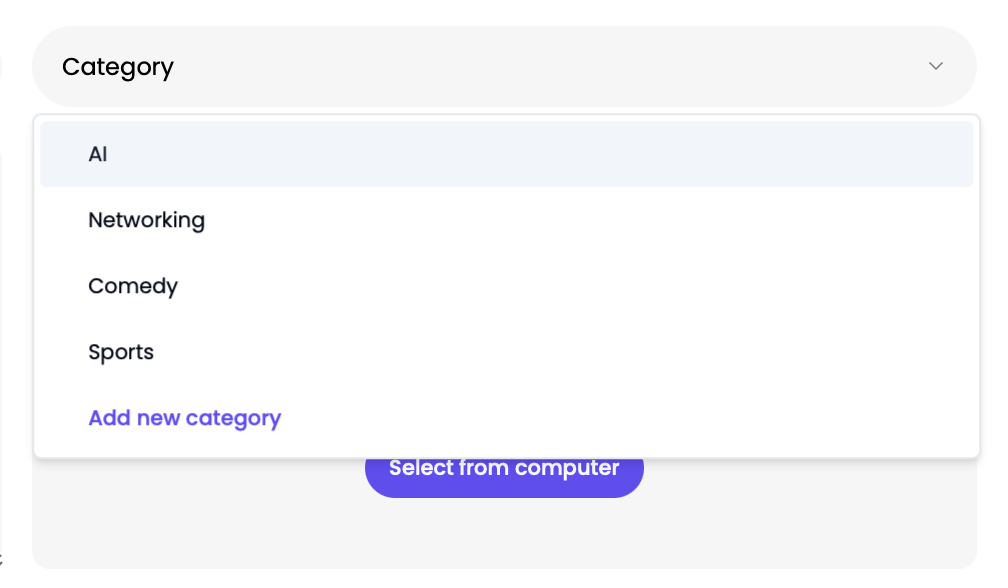
\includegraphics[width=0.6\textwidth,height=200px,frame]{images/createEvent2.png}
	\caption{Create Event - New Category}
        \label{fig:createEvent2}
\end{figure}


The features outlined in this manual are designed to ensure a seamless and intuitive user experience on the platform. By following the instructions in this guide, users can efficiently navigate the website and make the most of its functionalities. Additionally, the detailed sections allow users to troubleshoot and resolve any issues by referring directly to the relevant topics listed in the table of contents.

In the following section, the focus shifts to the \textbf{Developer's Guide}, providing an in-depth explanation of the platform's software implementation. This guide covers both the \textbf{front-end} and \textbf{back-end} systems, offering developers a comprehensive understanding of the platform's architecture, tools, and technologies to assist in further customization and maintenance.




% \begin{table}[H]
% 	\centering
% 	\begin{tabular}{ | m{0.25\textwidth} | m{0.65\textwidth} | }
% 		\hline
% 		\textbf{Phasellus tortor} & \textbf{Aenean consequat} \\
% 		\hline \hline
% 		\emph{Sed malesuada} & Aliquam aliquam velit in convallis ultrices. \\
% 		\hline
% 		\emph{Purus sagittis} &  Quisque lobortis eros vitae urna lacinia euismod. \\
% 		\hline
% 		\emph{Pellentesque} & Curabitur ac lacus pellentesque, eleifend sem ut, placerat enim. Ut auctor tempor odio ut dapibus. \\
% 		\hline
% 	\end{tabular}
% 	\caption{Maecenas tincidunt non justo quis accumsan}
% 	\label{tab:example-1}
% \end{table}

% \subsection{Multi rows and multi columns}

% Mauris a dapibus lectus. Vestibulum commodo nibh ante, ut maximus magna eleifend vel. Integer vehicula elit non lacus lacinia, vitae porttitor dolor ultrices. Vivamus gravida faucibus efficitur. Ut non erat quis arcu vehicula lacinia. Nulla felis mauris, laoreet sed malesuada in, euismod et lacus. Aenean at finibus ipsum. Pellentesque dignissim elit sit amet lacus congue vulputate.

% \begin{table}[htb]
% 	\centering
% 	\begin{tabular}{ | c | r | r | r | r | r | r | }
% 		\hline
% 		\multirow{2}{*}{\textbf{Quisque}} & \multicolumn{2}{ c | }{\textbf{Suspendisse}} & \multicolumn{2}{ c | }{\textbf{Aliquam}} & \multicolumn{2}{ c | }{\textbf{Vivamus}} \\
% 		\cline{2-7}
% 		& Proin & Nunc & Proin & Nunc & Proin & Nunc \\
% 		\hline \hline		
% 		Leo & 2,80 MB & 100\% & 232 KB & 8,09\% & 248 KB & 8,64\% \\
% 		\hline
% 		Vel & 9,60 MB & 100\% & 564 KB & 5,74\% & 292 KB & 2,97\% \\
% 		\hline
% 		Auge & 78,2 MB & 100\% & 52,3 MB & 66,88\% & 3,22 MB & 4,12\% \\
% 		\hline 
% 	\end{tabular}
% 	\caption[Rövid cím a táblázatjegyzékbe]{Vivamus ac arcu fringilla, fermentum neque sed, interdum erat. Mauris bibendum mauris vitae enim mollis, et eleifend turpis aliquet.}
% 	\label{tab:example-2}
% \end{table}

% \subsection{Long tables over multiple pages}

% Nunc porta placerat leo, sit amet porttitor dui porta molestie. Aliquam at fermentum mi. Maecenas vitae lorem at leo tincidunt volutpat at nec tortor. Vivamus semper lacus eu diam laoreet congue. Vivamus in ipsum risus. Nulla ullamcorper finibus mauris non aliquet. Vivamus elementum rhoncus ex ut porttitor.

% \begin{center}
% 	\begin{longtable}{ | p{0.3\textwidth} | p{0.7\textwidth} | }
		
% 		\hline
% 		\multicolumn{2}{|c|}{\textbf{Praesent aliquam mauris enim}}
% 		\\ \hline
		
% 		\emph{Suspendisse potenti} & \emph{Lorem ipsum dolor sit amet}
% 		\\ \hline \hline
% 		\endfirsthead % table header on first page
		
% 		\hline
% 		\emph{Suspendisse potenti} & \emph{Lorem ipsum dolor sit amet}
% 		\\ \hline \hline
% 		\endhead % table header on further pages
		
% 		\hline
% 		\endfoot % table footer on previous pages
		
% 		\endlastfoot % table footer on last page
		
% 		\emph{Praesent}
% 		& Nulla ultrices et libero sit amet fringilla. Nunc scelerisque ante tempus sapien placerat convallis.
% 		\\ \hline
		
% 		\emph{Luctus}
% 		& Integer hendrerit erat massa, non hendrerit risus convallis at. Curabitur ultrices, justo in imperdiet condimentum, neque tortor luctus enim, luctus posuere massa erat vitae nibh.
% 		\\ \hline
		
% 		\emph{Egestas}
% 		& Duis fermentum feugiat augue in blandit. Mauris a tempor felis. Pellentesque ultricies tristique dignissim. Pellentesque aliquam semper tristique. Nam nec egestas dolor. Vestibulum id elit quis enim fringilla tempor eu a mauris. Aliquam vitae lacus tellus. Phasellus mauris lectus, aliquam id leo eget, auctor dapibus magna. Fusce lacinia felis ac elit luctus luctus.
% 		\\ \hline
		
% 		\emph{Dignissim}
% 		& Praesent aliquam mauris enim, vestibulum posuere massa facilisis in. Suspendisse potenti. Nam quam purus, rutrum eu augue ut, varius vehicula tellus. Fusce dui diam, aliquet sit amet eros at, sollicitudin facilisis quam. Phasellus tempor metus vel augue gravida pretium. Proin aliquam aliquam blandit. Nulla id tempus mi. Fusce in aliquam tortor.
% 		\\ \hline
		
% 		\emph{Pellentesque}
% 		& Donec felis nibh, imperdiet a arcu non, vehicula gravida nibh. Quisque interdum sapien eu massa commodo, ac elementum felis faucibus.
% 		\\ \hline
		
% 		\emph{Molestie}
% 		& Cras ullamcorper tellus et auctor ultricies. Maecenas tincidunt euismod lectus nec venenatis. Suspendisse potenti. Pellentesque pretium nunc ut euismod cursus. Nam venenatis condimentum quam. Curabitur suscipit efficitur aliquet. Interdum et malesuada fames ac ante ipsum primis in faucibus.
% 		\\ \hline
		
% 		\emph{Vivamus semper}
% 		& In purus purus, faucibus eu libero vulputate, tristique sodales nunc. Nulla ut gravida dolor. Fusce vel pellentesque mi, vel efficitur eros. Nunc vitae elit tellus. Sed vestibulum auctor consequat. 
% 		\\ \hline
		
% 		\emph{Condimentum}
% 		& Nulla scelerisque, leo et facilisis pretium, risus enim cursus turpis, eu suscipit ipsum ipsum in mauris. Praesent eget pulvinar ipsum, suscipit interdum nunc. Nam varius massa ut justo ullamcorper sollicitudin. Vivamus facilisis suscipit neque, eu fermentum risus. Ut at mi mauris.
% 		\\ \hline
		
% 		\caption{Praesent ullamcorper consequat tellus ut eleifend}
% 		\label{tab:example-3}		
% 	\end{longtable}
% \end{center}